\notechapter{N-20240413}{Local Linear Geometry: Derivatives, Charts, and Tangent Spaces}

\section{Why this note belongs to geometry}

The derivative is often introduced as a rule for computing slopes. In several variables that description becomes too small. The derivative is really the first local geometric model of a map. Near a point \(p\), a smooth map behaves like a linear map:
\[
  f(p+h)=f(p)+Df_p(h)+\text{smaller error}.
\]
This is the bridge from calculus to differential geometry.

The guiding idea is:
\[
  \text{a curved object is understood by replacing it locally by its best linear shadow.}
\]
That shadow is the tangent space.

\begin{figure}[H]
\centering
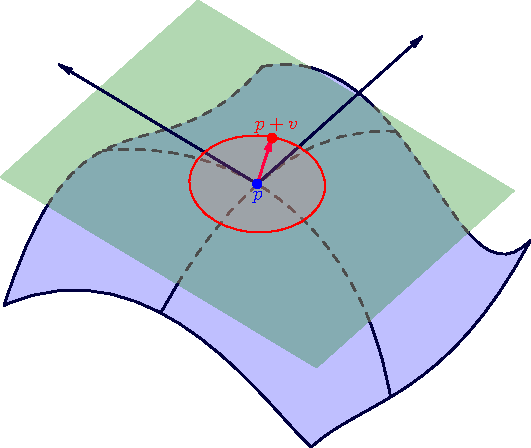
\includegraphics[width=.55\linewidth]{figures/N-20240413/tangent.pdf}
\caption{A tangent line is the first local linear model of a curve.}
\end{figure}

\section{The total derivative}

Let \(f:\mathbb R^n\to\mathbb R^m\). The total derivative at \(p\) is the linear map
\[
  Df_p:\mathbb R^n\to\mathbb R^m
\]
which best approximates \(f\) near \(p\):
\[
  f(p+h)=f(p)+Df_p(h)+o(\|h\|).
\]
The important word is \emph{linear}. Partial derivatives are not separate pieces of magic. They are the coordinates of this one linear map.

If \(f=(f_1,\ldots,f_m)\), the matrix of \(Df_p\) is the Jacobian
\[
  J_f(p)=
  \begin{bmatrix}
  \partial f_1/\partial x_1&\cdots&\partial f_1/\partial x_n\\
  \vdots&\ddots&\vdots\\
  \partial f_m/\partial x_1&\cdots&\partial f_m/\partial x_n
  \end{bmatrix}_{p}.
\]
So the derivative is not the matrix itself; the matrix is how the linear map looks after choosing coordinates.

\section{The chain rule as geometry}

If
\[
  \mathbb R^n\xrightarrow{f}\mathbb R^m\xrightarrow{g}\mathbb R^k,
\]
then
\[
  D(g\circ f)_p=Dg_{f(p)}\circ Df_p.
\]
This is the chain rule. In coordinates it becomes matrix multiplication, but the geometric meaning is simpler: local linear approximations compose.

\section{Tangent planes}

For a graph \(z=f(x,y)\), the tangent plane at \((a,b,f(a,b))\) is
\[
  z=f(a,b)+f_x(a,b)(x-a)+f_y(a,b)(y-b).
\]
This says that the graph is locally approximated by an affine plane whose direction is controlled by \(Df_{(a,b)}\).

For a level surface \(F(x,y,z)=c\), the tangent plane at \(p\) is
\[
  \nabla F(p)\cdot (X-p)=0.
\]
Here \(\nabla F(p)\) is normal to the surface. Again, the local geometry is encoded by a first derivative.

\section{Manifolds in one page}

A manifold is a space that may be curved globally but looks Euclidean locally. A chart is a coordinate system on a small open piece:
\[
  \varphi:U\to \mathbb R^n.
\]
An atlas is a collection of charts covering the space. The transition maps \(\psi\circ\varphi^{-1}\) compare coordinates on overlaps. If these transition maps are smooth, the manifold is a smooth manifold.

Examples include
\[
  S^1,\quad S^2,\quad T^2,\quad \mathbb{RP}^n,\quad \mathbb{CP}^n.
\]
Each is locally Euclidean, but none should be mistaken for a single Euclidean coordinate patch.

\section{Tangent vectors}

There are two useful pictures of tangent vectors. First, a tangent vector is the velocity of a curve:
\[
  v=\gamma'(0),\qquad \gamma(0)=p.
\]
Second, a tangent vector is a directional derivative acting on functions:
\[
  v(f)=\left.\frac{d}{dt}\right|_{t=0}f(\gamma(t)).
\]
The second viewpoint is more intrinsic. It does not require the manifold to sit inside a larger Euclidean space.

The tangent space \(T_pM\) is the vector space of tangent vectors at \(p\). A smooth map \(F:M\to N\) induces a linear map
\[
  dF_p:T_pM\to T_{F(p)}N.
\]
This is the manifold version of the total derivative.

\section{Regular values make manifolds}

Suppose \(F:\mathbb R^n\to\mathbb R^k\) is smooth. If \(c\) is a regular value, meaning \(DF_p\) is surjective for every \(p\in F^{-1}(c)\), then
\[
  F^{-1}(c)
\]
is a smooth manifold of dimension \(n-k\).

For example,
\[
  S^2=\{(x,y,z):x^2+y^2+z^2=1\}
\]
is the level set of \(F(x,y,z)=x^2+y^2+z^2\). Since \(\nabla F=2(x,y,z)\) never vanishes on \(S^2\), the sphere is a smooth surface.

%% expanded-on-review

\section{A worked example: polar coordinates}

Consider the coordinate map
\[
  F(r,\theta)=(r\cos\theta,r\sin\theta).
\]
Its derivative is
\[
  DF_{(r,\theta)}=
  \begin{bmatrix}
  \cos\theta&-r\sin\theta\\
  \sin\theta&r\cos\theta
  \end{bmatrix}.
\]
The two columns have a direct geometric meaning:
\[
  \frac{\partial F}{\partial r}=(\cos\theta,\sin\theta),
  \qquad
  \frac{\partial F}{\partial\theta}=(-r\sin\theta,r\cos\theta).
\]
The first vector points outward. The second vector points along the circle of radius \(r\). This is exactly what a coordinate system should do: it translates coordinate motion into actual tangent motion.

This example also explains why coordinate formulas can be misleading. The symbols \(\partial/\partial r\) and \(\partial/\partial\theta\) are coordinate directions, but after applying the derivative they become concrete tangent vectors in the plane.

\section{The tangent space of the sphere}

For the sphere
\[
  S^2=\{x\in\mathbb R^3:\|x\|^2=1\},
\]
the tangent space at \(p\in S^2\) is
\[
  T_pS^2=\{v\in\mathbb R^3:p\cdot v=0\}.
\]
This follows by differentiating the constraint \(x\cdot x=1\). If \(\gamma(t)\subset S^2\) and \(\gamma(0)=p\), then
\[
  \gamma(t)\cdot\gamma(t)=1.
\]
Differentiating at \(t=0\) gives
\[
  2p\cdot\gamma'(0)=0.
\]
So every velocity vector is perpendicular to the radius vector.

This calculation is a good model for many geometric arguments: start from an equation defining the space, differentiate the equation, and obtain the linear equation defining the tangent space.

\section{A small warning about coordinates}

A chart is a language. It is not the object itself. The same tangent vector can have different coordinate descriptions in different charts. What should remain unchanged is the geometric vector, not its coordinate list.

This is why differential geometry tries to separate intrinsic statements from coordinate expressions. Coordinates are useful for computation, but the real content is the object that survives changing coordinates.


\section{What to remember}

The derivative is the local linearization of geometry. The tangent space is the place where this linearization lives. A manifold is a space that allows this idea to be used locally everywhere.

The slogan is:
\[
\begin{array}{c}
  \text{calculus differentiates functions;}\\
  \text{geometry differentiates spaces.}
\end{array}
\]
